\chapter{Methods}\label{chap:methods}

\section{Setup}
We decided to install the project on an online web server and use it publically. 
This method will help all team members to work in the same area. 
In addition, this helped us to save more time.
The url for the project is \url{https:\\bank.atiqullah.dev}

\section{Client/Server Side Scripting }

One common client-side mechanism used to protect the login process is JavaScript form validation. 
This mechanism ensures that the user inputs valid data before the form is submitted to the server. 
For example, the JavaScript code may check that the username and password fields are not empty, 
that the password meets certain complexity requirements, or that an email address is properly formatted.

The fundamental security issue with client-side validation is that it can be easily bypassed. 
Since the validation code runs in the user's browser, a malicious user can disable or alter it using browser developer tools or by intercepting and modifying the HTTP requests. 
This means that relying solely on client-side validation for security is ineffective because it does not provide any protection against users who intentionally bypass the checks.

Steps to Circumvent JavaScript Form Validation:

\begin{enumerate}
    \item Open Developer Tools:
        \begin{itemize}
            \item Most modern browsers (Chrome, Firefox, Edge) have built-in developer tools that can be accessed by right-clicking on the web page and selecting "Inspect" or pressing Ctrl+Shift+I (Windows) or Cmd+Opt+I (Mac).
        \end{itemize}
    \item Locate the Login Form:
        \begin{itemize}
            \item Use the Elements tab to locate the HTML form element for login. This can usually be done by searching for <form> tags.
        \end{itemize}
    \item Disable JavaScript Validation:
        \begin{itemize}
            \item Remove the onsubmit attribute from the form tag if it is calling a JavaScript function for validation.
            \item Alternatively, navigate to the Sources tab, find the JavaScript file containing the validation code, and either comment out or modify the relevant validation logic.
        \end{itemize}
    \item Manually Submit the Form:
        \begin{itemize}
            \item Fill in the form fields with the desired values and submit the form manually using the browser.
        \end{itemize}
    \item Intercept and Modify HTTP Requests (Optional):
        \begin{itemize}
            \item Use tools like OWASP ZAP and Burp Suite or browser extensions like Tamper Data to intercept the HTTP request and modify it before it reaches the server.
        \end{itemize}
\end{enumerate}

To prevent this, one of the better solutions is \textbf{Server-Side Validation and Security Measures}:
To ensure the security of the login process, the following steps should be taken:
\begin{enumerate}
\item Server-Side Validation:
        \begin{itemize}
            \item Implement validation checks on the server side to ensure that all input data is valid and meets the requirements. This prevents users from bypassing the validation.
        \end{itemize}
\item Use HTTPS:
    \begin{itemize}
        \item Encrypt the communication between the client and the server using HTTPS to protect the data in transit, especially login credentials.
    \end{itemize}
\item Rate Limiting and Account Lockout:
    \begin{itemize}
        \item Implement rate limiting to prevent brute-force attacks. After a certain number of failed login attempts, temporarily lock the account or require additional verification.
    \end{itemize}
\item Multi-Factor Authentication (MFA):
    \begin{itemize}
        \item Add an extra layer of security by requiring a second form of authentication, such as a one-time password (OTP) sent to the user's mobile device.
    \end{itemize}
\item Secure Password Storage:
    \begin{itemize}
        \item Store passwords securely using hashing algorithms such as bcrypt, scrypt, or Argon2. Never store plain-text passwords.
    \end{itemize}
\item CSRF Protection:
    \begin{itemize}
        \item Implement Cross-Site Request Forgery (CSRF) protection to prevent unauthorized commands from being transmitted from a user that the web application trusts.
    \end{itemize}
\end{enumerate}
By implementing these server-side security measures, we can significantly enhance the security of the login process and protect against various types of attacks.


\section{SQL Injection}
Before conducting a penetration test on a vulnerable host, it is essential to identify the Database Management System (DBMS) that the host is running. 
Understanding the system's specifications provides valuable insights. Notably, the eregi() function was deprecated in PHP version 5.3 and replaced with the preg\_match() function, indicating the use of PHP version 5.3.

To identify potential SQL injection vulnerabilities, our approach involves testing the application's input fields with basic SQL injection payloads. 
We begin with simple SQL operands such as '', OR '1'='1', and AND '1'='1'. 
These payloads help in determining if the application is susceptible to SQL injection attacks. 
By systematically testing these basic operands, we can observe the application's behavior and responses, which will guide us in refining our injection techniques and understanding the underlying DBMS. 
This methodical approach ensures we gather the necessary information to exploit vulnerabilities effectively and safely.

\begin{figure}[H]
    \centering
    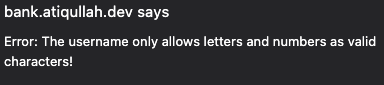
\includegraphics[width=0.5\linewidth]{image13.png}
    \caption{Invalid Username and Password Response}
    \label{fig:image13}
\end{figure}

\subsection{Observation}
Response \ref{fig:image13} from the server indicates that input fields use proper validation handling and successfully filter out special characters. 
The application is still potentially vulnerable to SQL injection even with input field sanitization
We will try to log in without knowing the password and bypass the login authentication system. 

\subsection{Injection on login}
After observing the HTML code of the page with the help of browser Inspect Elements, we removed the \textbf{onclick} parameter from the button tag. 
In addition, we change the button type from button to submit. 
With these changes, we can bypass the JavaScript validation and submit the request directly to the server. Figure \ref{fig:loginFormChanges} shows the changes.
\begin{figure}[H]
    \centering
    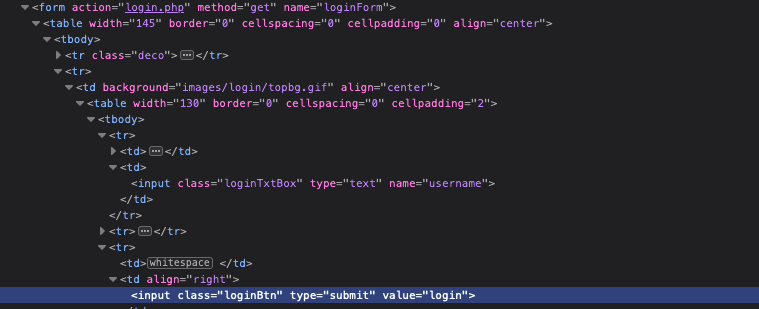
\includegraphics[width=0.5\linewidth]{alisina/changesOnLoginForm.png}
    \caption{Changes on Login Form}
    \label{fig:loginFormChanges}
\end{figure}
First, we called the \textbf{login.php} directly. In response, we received the server error message and column name which is shown in figure \ref{fig:LoginFormErrorWithColumns}.
\begin{figure}[H]
    \centering
    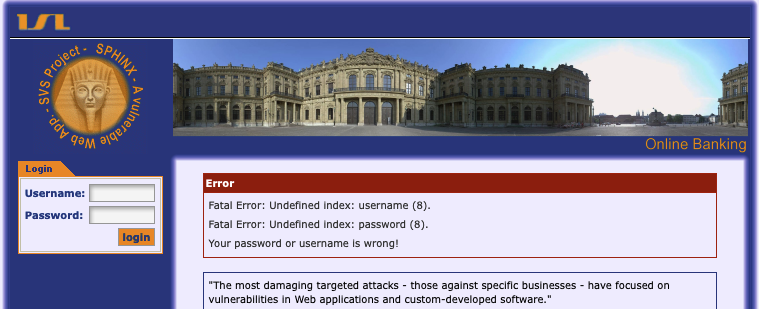
\includegraphics[width=0.5\linewidth]{alisina/LoginFormErrorWithColumns.png}
    \caption{Login Error}
    \label{fig:LoginFormErrorWithColumns}
\end{figure}

Then, we inject the boolean injection method which is inserting \textit{OR '1'='1' \#, and AND '1'='1' \#} to the first text field which is the username in our case. \# at the indicates that comment whatever after this.
After injection, we successfully managed to bypass the login screen and log in as the first user which is Alex. 
Figure \ref{fig:loggedInUser} shows the successful login without credentials.

\begin{figure}[H]
    \centering
    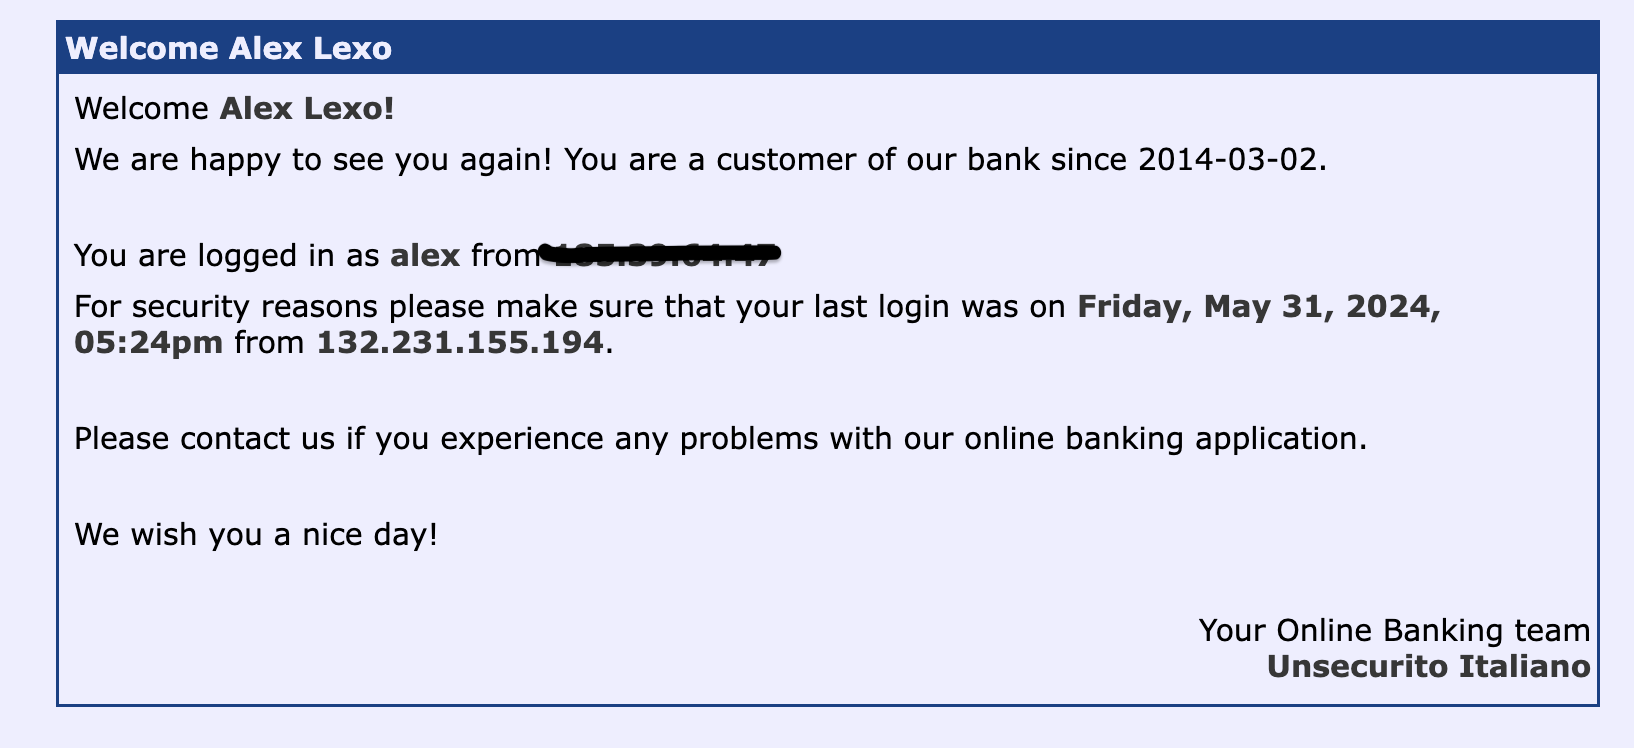
\includegraphics[width=0.5\linewidth]{image6.png}
    \caption{By Passed Authentication Page}
    \label{fig:loggedInUser}
\end{figure}

\subsection{Injection on change password}
To change the user's password through the SQL injection we need to check change password page is injectable or not.
After passing malicious characters to the input fields and submitting them to the server we have found out that the system validates the input on the server side and it is returning errors along with the invalid password. 
This indicates that the change password URL is injectable. Figure \ref{fig:invalidPasswordResponse} shows the response along with the error.
\begin{figure}[H]
    \centering
    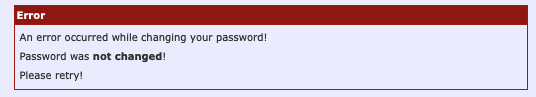
\includegraphics[width=0.5\linewidth]{alisina/changepassworderror.png}
    \caption{Invalid Password Response}
    \label{fig:invalidPasswordResponse}
\end{figure}

To change the password without knowing the old password we inject a malicious query \textbf{' OR 1=1 -- } to the old password text field, set the new password, and confirm the password to "test". 
It is good to mention that we have added one space after \textbf{--} in the malicious query.
In addition with the help of the browser's Inspect Elements, we changed all three text fields from password to text. 
These changes helped us to see our input data.
The Figure \ref{fig:ChangePasswordInjection} shows the our input.
\begin{figure}[H]
    \centering
    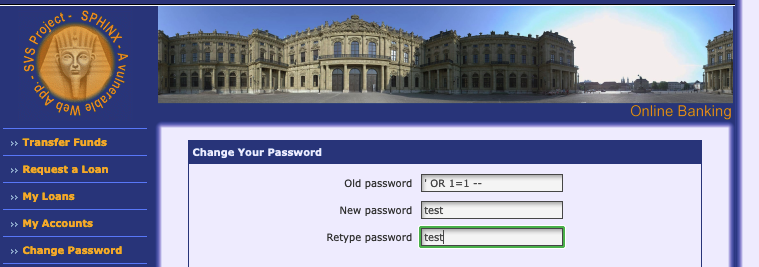
\includegraphics[width=0.5\linewidth]{alisina/ChangePasswordInjection.png}
    \caption{Change Password Injection}
    \label{fig:ChangePasswordInjection}
\end{figure}

\subsection{User Creation}
Creating a new user in the system requires knowing the type of DBMS, database name, table name, and column name. 
To receive the mentioned details we have used SQLMap.
SQLMap is an open-source penetration testing tool that automates the process of detecting and exploiting SQL injection flaws and taking over database servers.
We have targeted the login URL to test in SQL map, we did not perform an injectable check due to we already knew about it in the previous steps.
\begin{itemize}
    \item Database type and name, the figure \ref{fig:dbname} shows how to find the Database type and name with SQLMap. 
        \begin{figure}[H]
            \centering
            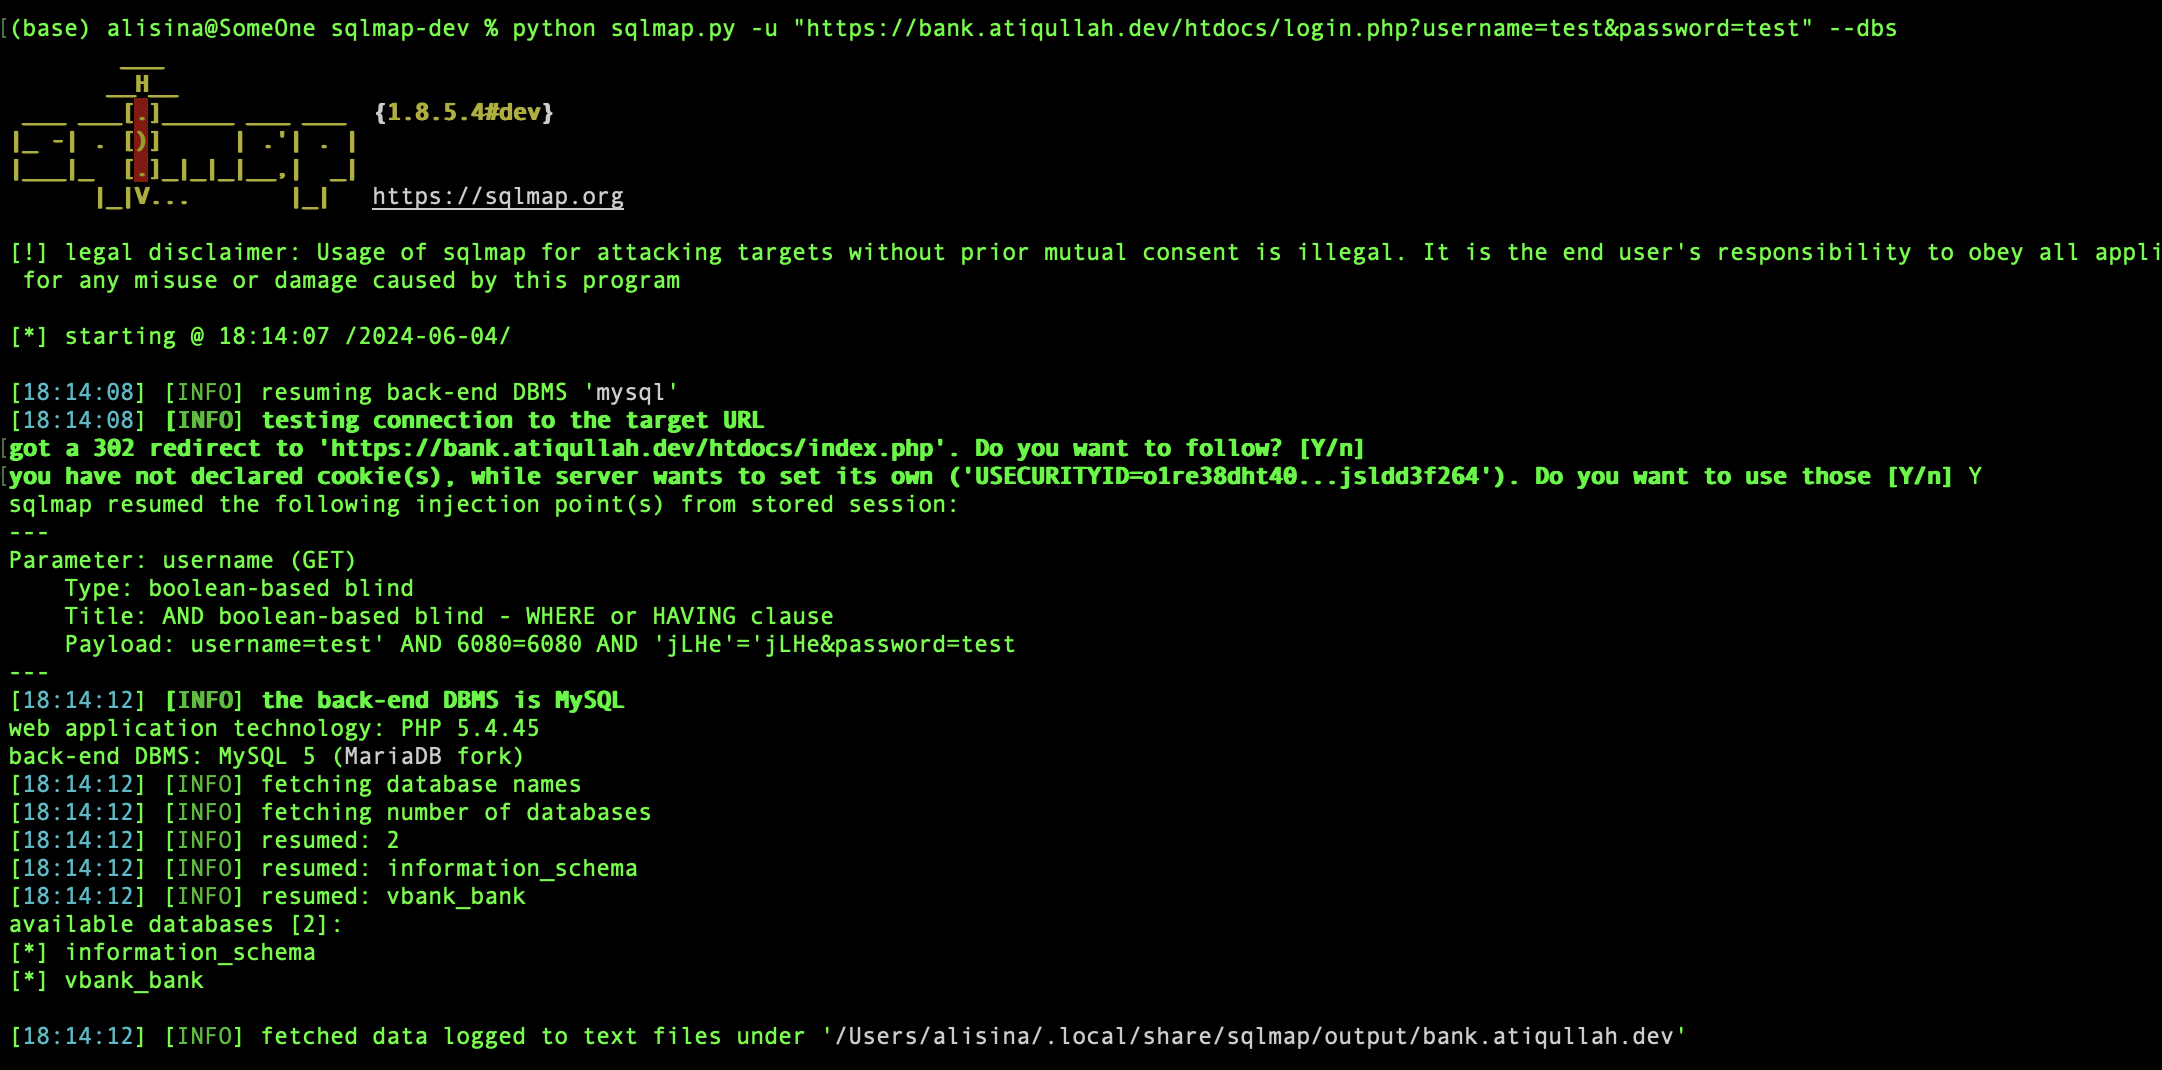
\includegraphics[width=0.9\linewidth]{alisina/sqlmapDBNAME.png}
            \caption{Database type and name}
            \label{fig:dbname}
        \end{figure}
    \item Tables, table columns. Figure \ref{fig:allInfoQeurySQLMAP} shows the query. Figure \ref{fig:dbTBs} shows the tables. Figure \ref{fig:userTableCol} shows the \textbf{users} table columns.
        \begin{figure}[H]
            \centering
            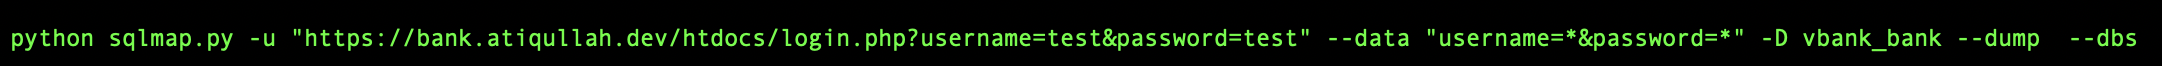
\includegraphics[width=0.9\linewidth]{alisina/DBallQeury.png}
            \caption{Qeury for information retrieval.}
            \label{fig:allInfoQeurySQLMAP}
        \end{figure}
        \begin{figure}[H]
            \centering
            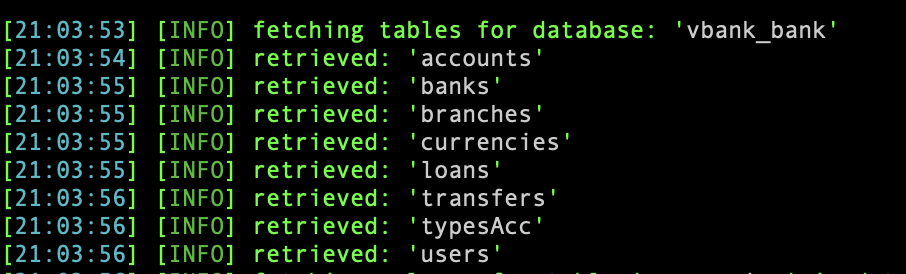
\includegraphics[width=0.9\linewidth]{alisina/DbTables.png}
            \caption{Database Tables}
            \label{fig:dbTBs}
        \end{figure}
        \begin{figure}[H]
            \centering
            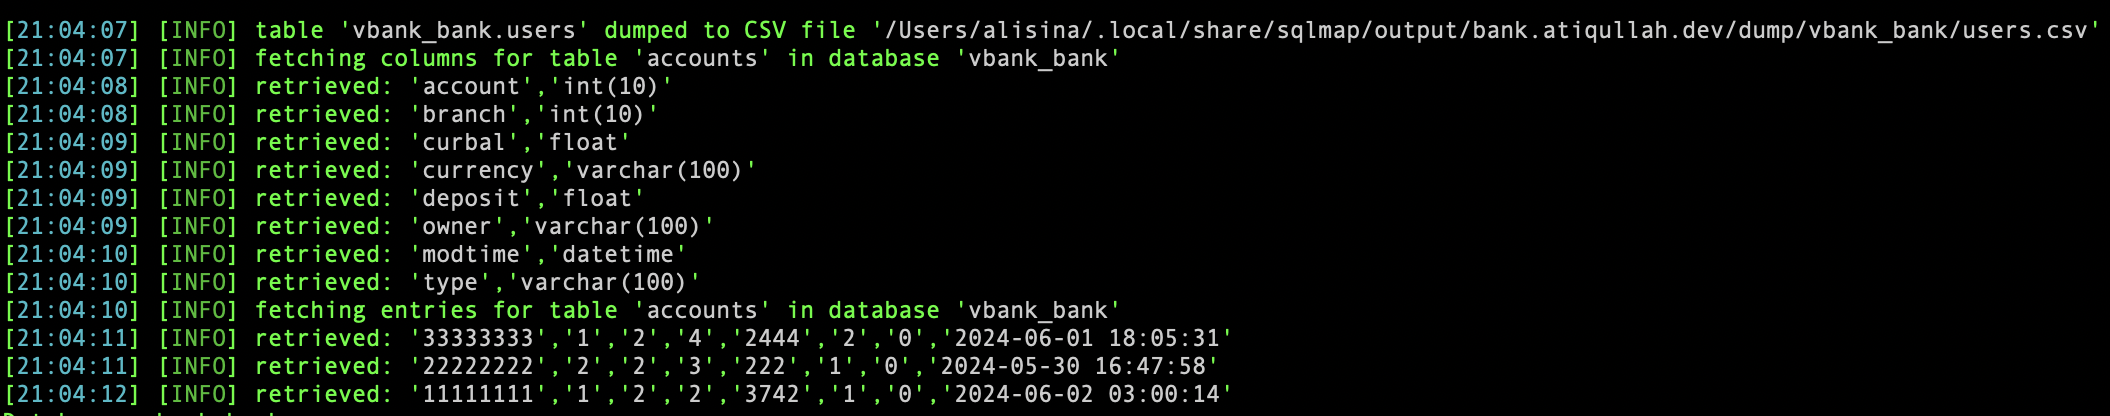
\includegraphics[width=0.9\linewidth]{alisina/DBUSERS.png}
            \caption{User table columns}
            \label{fig:userTableCol}
        \end{figure}
\end{itemize}

We have found out that the DBMS is \textbf{MySQL} and database name is \textbf{vbank\_bank}, user account table is \textbf{users}.
To create a new user we injected the following query along the with login URL which is shown in figure \ref{fig:insertQeury}.
\begin{figure}[H]
    \centering
    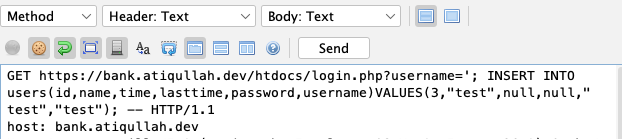
\includegraphics[width=0.9\linewidth]{alisina/InsertQuery.png}
    \caption{Insert Query to create user}
    \label{fig:insertQeury}
\end{figure}
Figure \ref{fig:testUser} shows that the new user logged in to the system.
\begin{figure}[H]
    \centering
    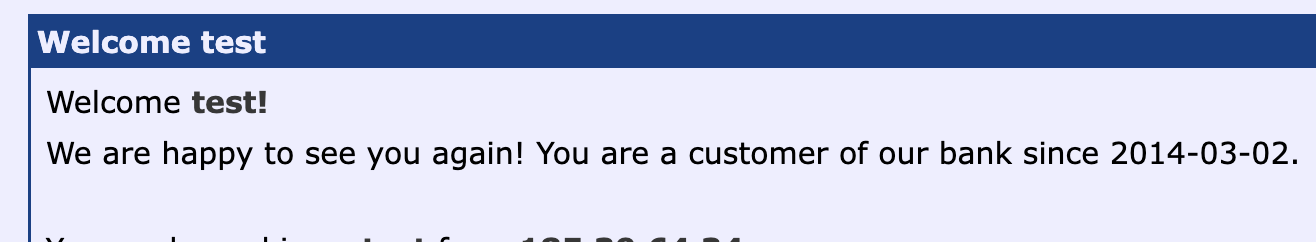
\includegraphics[width=0.9\linewidth]{image8.png}
    \caption{"Test" user after logged in}
    \label{fig:testUser}
\end{figure}

\subsection{Request Manipulation }
For request manipulation, we have used to software Burp Suite and OWASP ZAP. For this part of the exercise, we used Burp Suit.
Using Burp Suite, we can exploit a Cross-Site Request Forgery (CSRF) vulnerability to transfer funds to a malicious user's account. 
First, we intercept a legitimate request to transfer funds within the bank application. Figure \ref{fig:legitimateTransfer} shows a legitimate transfer page.
This request typically includes parameters such as the sender's account number, the recipient's account number, and the transfer amount. 
By capturing this request with Burp Suite, we can identify the specific parameters and the request format. 
Next, we craft a malicious request that mimics the legitimate transfer request but redirects the funds to an account controlled by the attacker. 
We then create a malicious web page containing an HTML form that, when visited by the victim, automatically submits the crafted request without the victim’s knowledge. 
By leveraging Burp Suite's features we ensure it bypasses any client-side protections. 
When the victim, who is authenticated in their banking session, unknowingly visits the malicious page, the crafted request is executed, transferring the funds to the attacker's account. 
This demonstrates how Burp Suite can be used to identify and exploit CSRF vulnerabilities to perform unauthorized actions on behalf of unsuspecting users.

First, we need to identify the structure of the URL and continue with the CSRF exploit:
\begin{figure}[H]
    \centering
    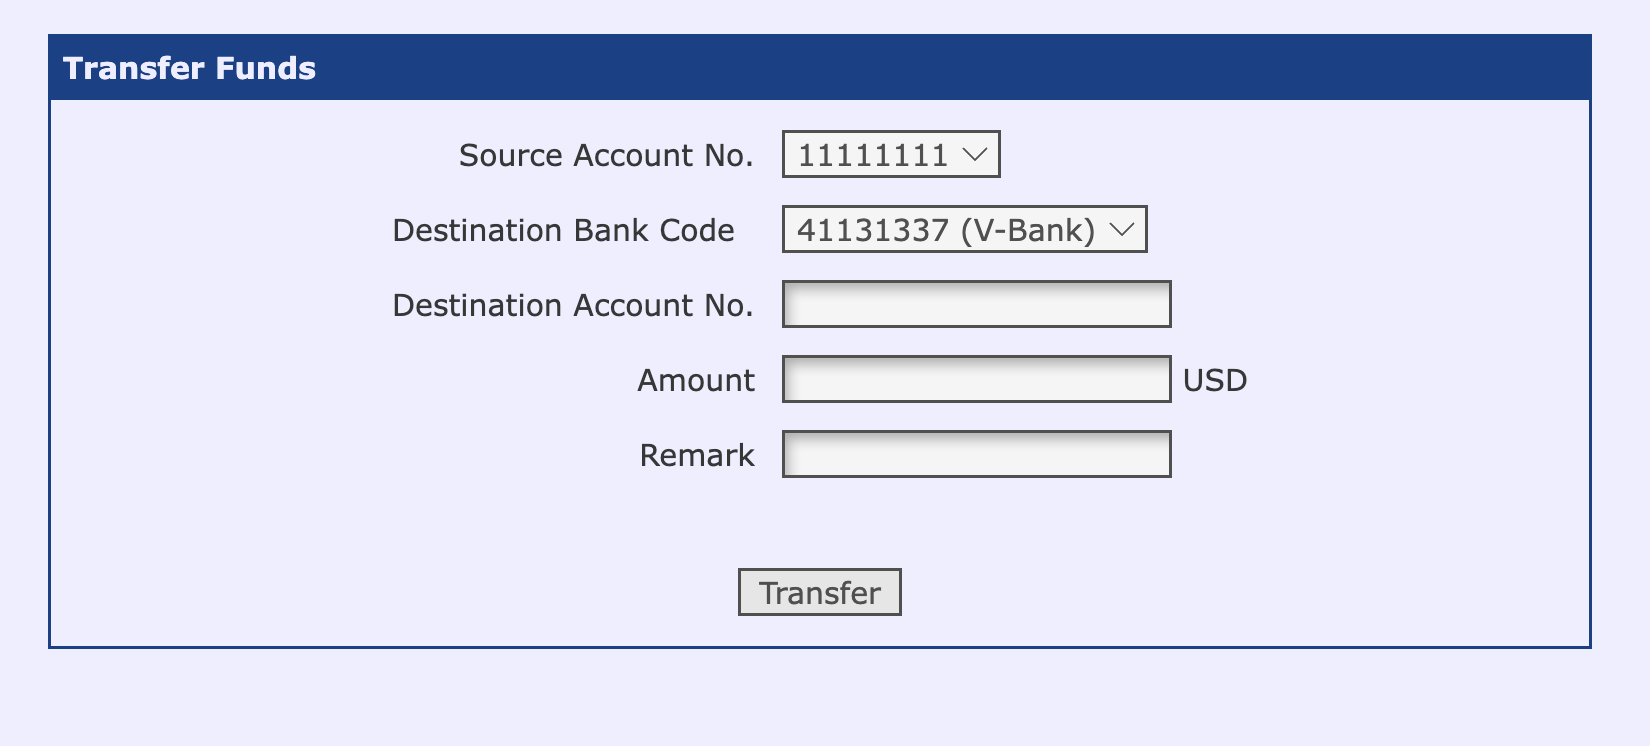
\includegraphics[width=0.9\linewidth]{image15.png}
    \caption{Transfer view}
    \label{fig:legitimateTransfer}
\end{figure}

\begin{figure}[H]
    \centering
    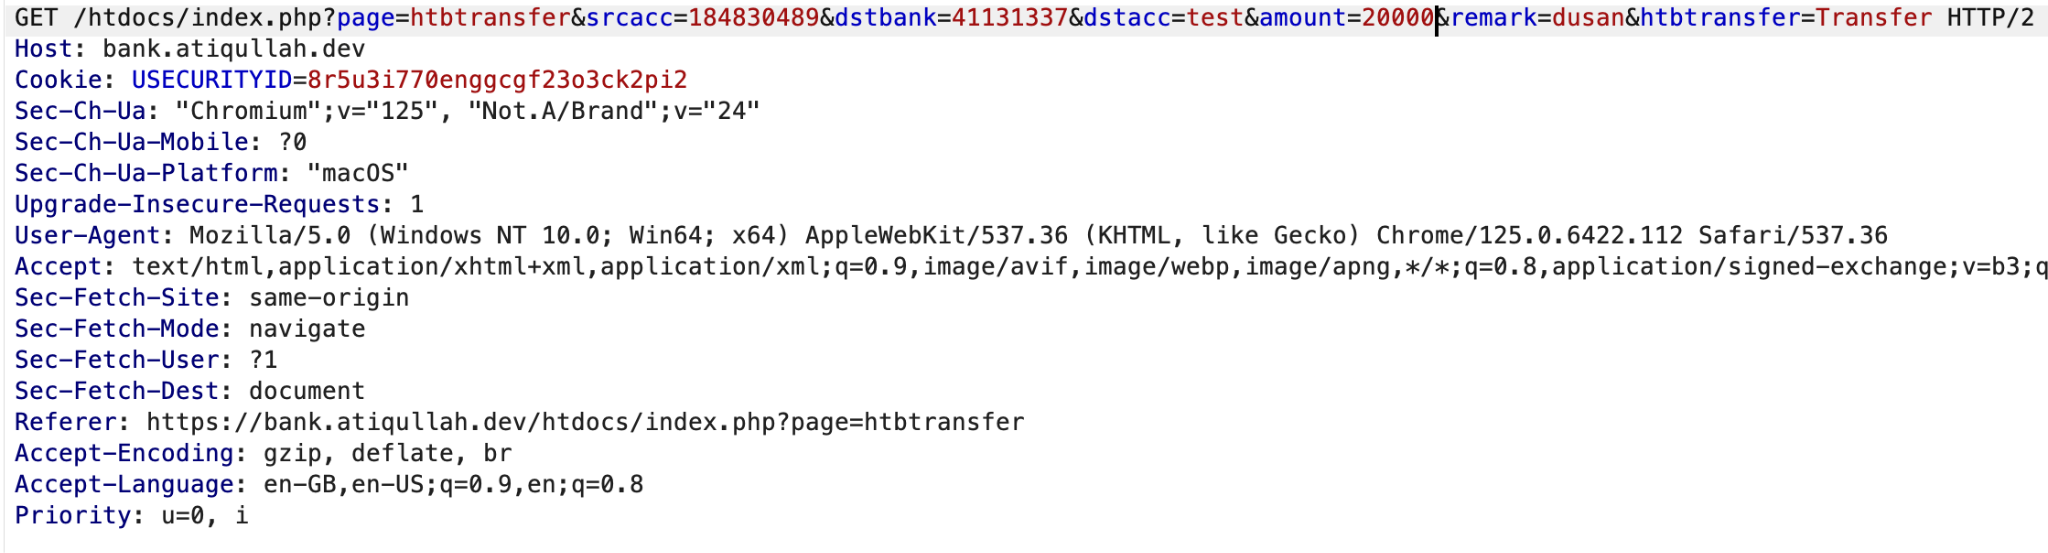
\includegraphics[width=0.9\linewidth]{image2.png}
    \caption{Intercepted Transfer Data}
    \label{fig:interceptedTransferData}
\end{figure}
We intercepted a request \ref{fig:interceptedTransferData} to transfer funds within the bank application, revealing the critical parameters involved in the transaction. 
The captured request was: 
\begin{tiny}
    \begin{verbatim}
 GET /htdocs/index.php?page=htbtransfer\&srcacc=184830489\&dstbank=41131337\&dstacc=test\&amount=20000\&remark=dusan\&
 htbtransfer=Transfer HTTP/2. 
    \end{verbatim}
\end{tiny}

This request includes several parameters: srcacc (source account number), dstbank (destination bank code), dstacc (destination account number), amount (transfer amount), remark (transaction remark), and htbtransfer (action to initiate the transfer). By analyzing this request, we understood the structure and flow of the transaction. We then modified the intercepted request to redirect the funds to a malicious user. Specifically, we changed the dstacc parameter to reflect the attacker's account number, for instance, dstacc=123456789. The modified request thus became: 
\begin{tiny}
\begin{verbatim} 
 GET /htdocs/index.php?page=htbtransfer&srcacc=184830489&dstbank=41131337&dstacc=123456789&amount=20000&remark=dusan&
 htbtransfer=Transfer HTTP/2. 
\end{verbatim}
\end{tiny}

This alteration ensures that when the request is processed by the server, the \$20,000 transfer is directed to the attacker’s account instead of the intended recipient. Figure \ref{fig:interceptedTransferDataChanged} shows changes in intercepted transactions.
\begin{figure}[H]
    \centering
    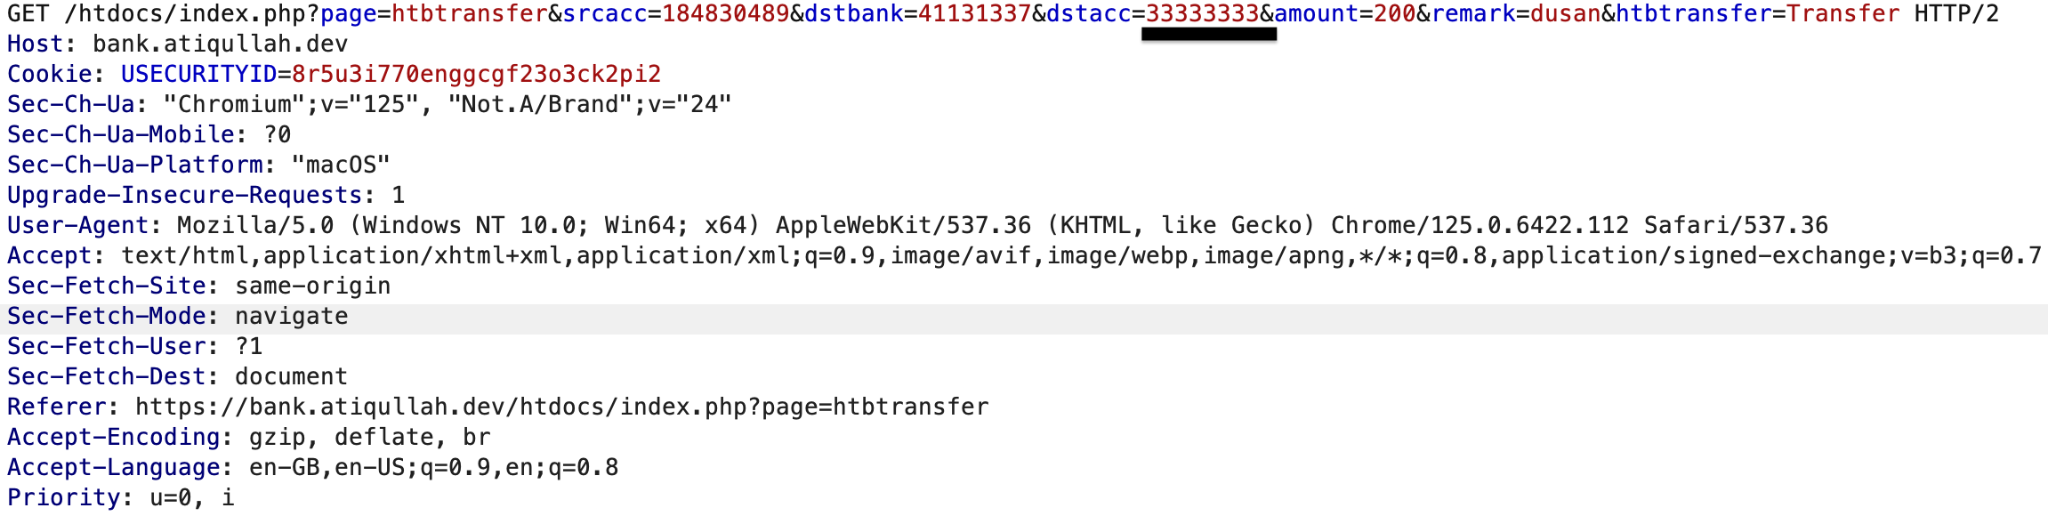
\includegraphics[width=0.9\linewidth]{image3.png}
    \caption{Intercepted Transfer Data Changed}
    \label{fig:interceptedTransferDataChanged}
\end{figure}

Furthermore, we modified the intercepted request to redirect the funds to a malicious user, ensuring that the dstacc parameter reflected an account number already existing in the system and adjusting the amount parameter to \$200 to comply with the user's available balance.
\begin{tiny}
\begin{verbatim} 
 /htdocs/index.php?page=htbtransfer&srcacc=184830489&dstbank=41131337&dstacc=33333333&amount=200&remark=dusan&
 htbtransfer=Transfer HTTP/2. 
\end{verbatim}
\end{tiny}

\subsubsection{Preventing CSRF}
Preventing Cross-Site Request Forgery (CSRF) attacks in PHP involves generating and validating CSRF tokens for form submissions. 
When the form is submitted, the server checks that the token matches the one stored in the user's session. 
This ensures that the request is genuine and originated from the authenticated user, not an attacker.


Code example:
\begin{verbatim}
session_start(); 
if (empty($_SESSION['csrf_token'])) {
 $_SESSION['csrf_token'] = bin2hex(random_bytes(32));
 }
\end{verbatim}


Some PHP libraries like Laravel already support CSRF token generation in their classes. 
Furthermore, we can take this route to follow the best security practices for our applications and prevent security risks. 

\subsection{Cross Site Scripting -XSS}
DOM-based Cross-Site Scripting (XSS) is a type of XSS attack that occurs when the client-side script of a web application manipulates the DOM (Document Object Model) in an insecure way, leading to the execution of malicious scripts. 
Unlike traditional XSS, where the payload is injected into the server response, DOM-based XSS happens entirely on the client side. 
This means that the malicious code is introduced and executed within the browser, without the server ever being aware of the attack.
The attack typically begins when an attacker crafts a malicious URL or injects malicious scripts into an existing page. 
This URL is then sent to the victim, often through social engineering techniques like phishing. 
When the victim clicks on the link, the browser loads the legitimate web page but with a malicious script embedded in it. 
The client-side JavaScript then reads data from the URL, such as parameters, fragments, or other parts of the DOM, and processes it in an insecure way, such as by using eval(), innerHTML, or other methods that directly inject content into the DOM without proper validation or escaping.
For example, if a web page includes a script that reads a query parameter from the URL and directly writes it to the page without sanitization, an attacker can exploit this by creating a URL that contains a script tag. 
When the victim loads this URL, the malicious script gets executed in their browser, allowing the attacker to perform actions like stealing cookies, session tokens, or other sensitive information, and even controlling the victim's interactions with the web application.

To Achieve we have used the BeEF XSS framework \nocite{beefproject}. BeEF is short for The Browser Exploitation Framework. It is a penetration testing tool that focuses on the web browser.

Through the interface of BeEF, we submit our script to target the web page. Figure \ref{fig:beefForst} shows the submitted JavaScript code in to web page.
\begin{figure}[H]
    \centering
    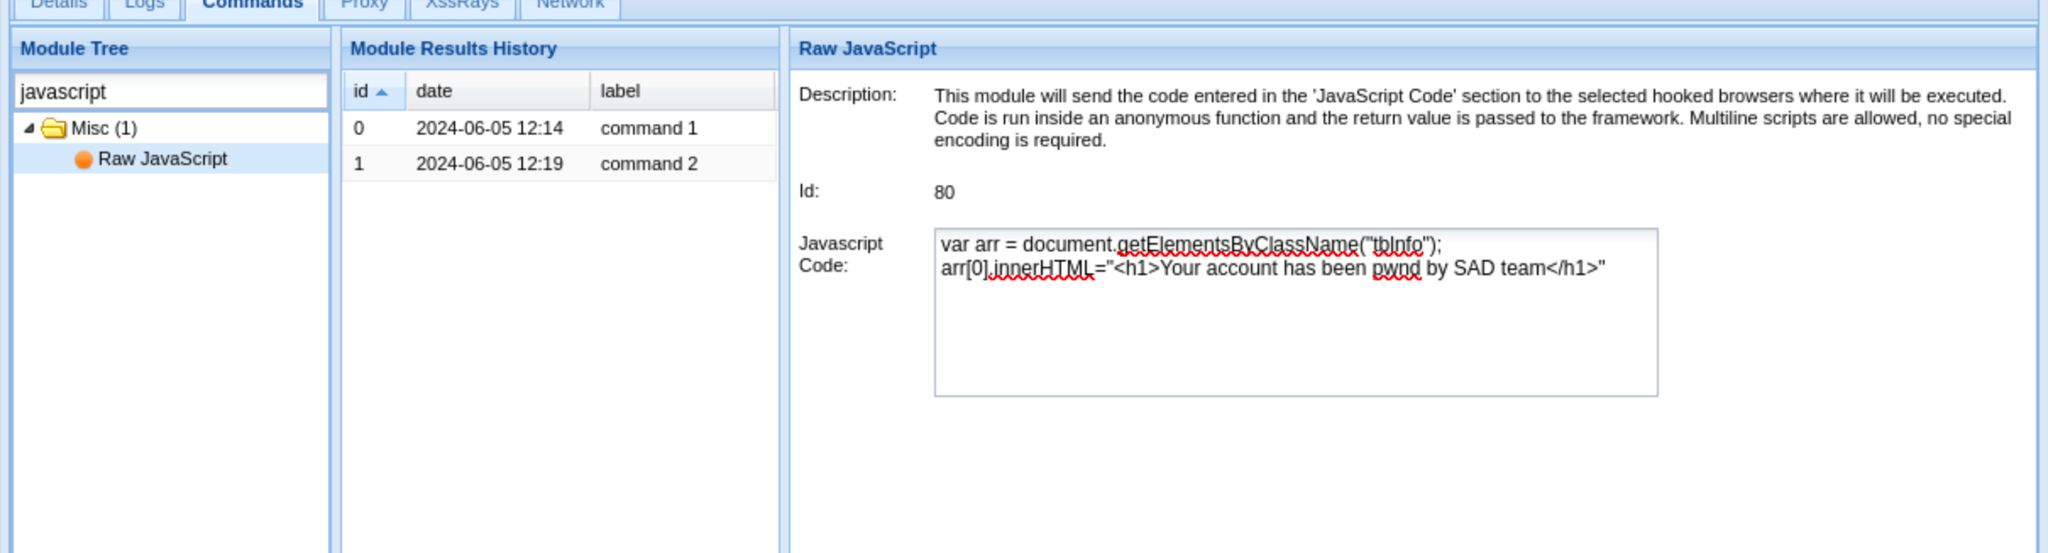
\includegraphics[width=0.7\linewidth]{alisina/BeefJavaScrit1.jpeg}
    \caption{JavaScript script through BeEF}
    \label{fig:beefForst}
\end{figure}

After submitting the script the users will see the message the in their web page. Figure \ref{fig:beefFirstResult} shows the result of attack.
\begin{figure}[H]
    \centering
    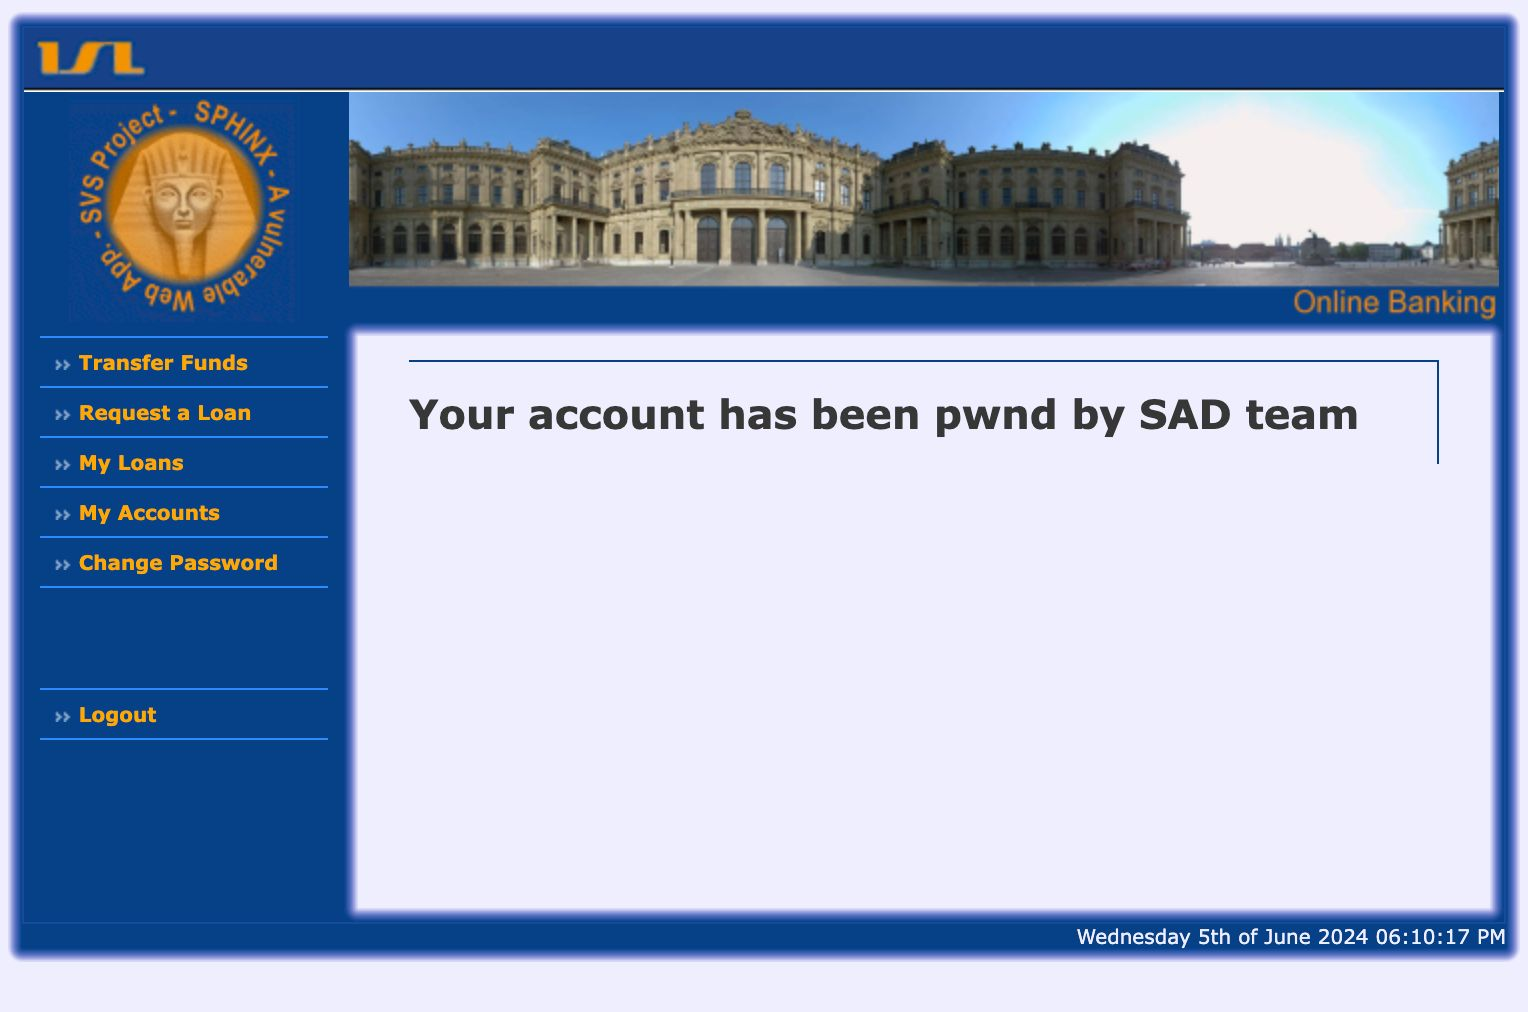
\includegraphics[width=0.7\linewidth]{alisina/beefResult1.jpeg}
    \caption{JavaScript script through BeEF}
    \label{fig:beefFirstResult}
\end{figure}

We did a DOM Request as an image tag to do unauthorized transactions from the user session which is shown in figure \ref{fig:beefImageTransaction}.
\begin{figure}[H]
    \centering
    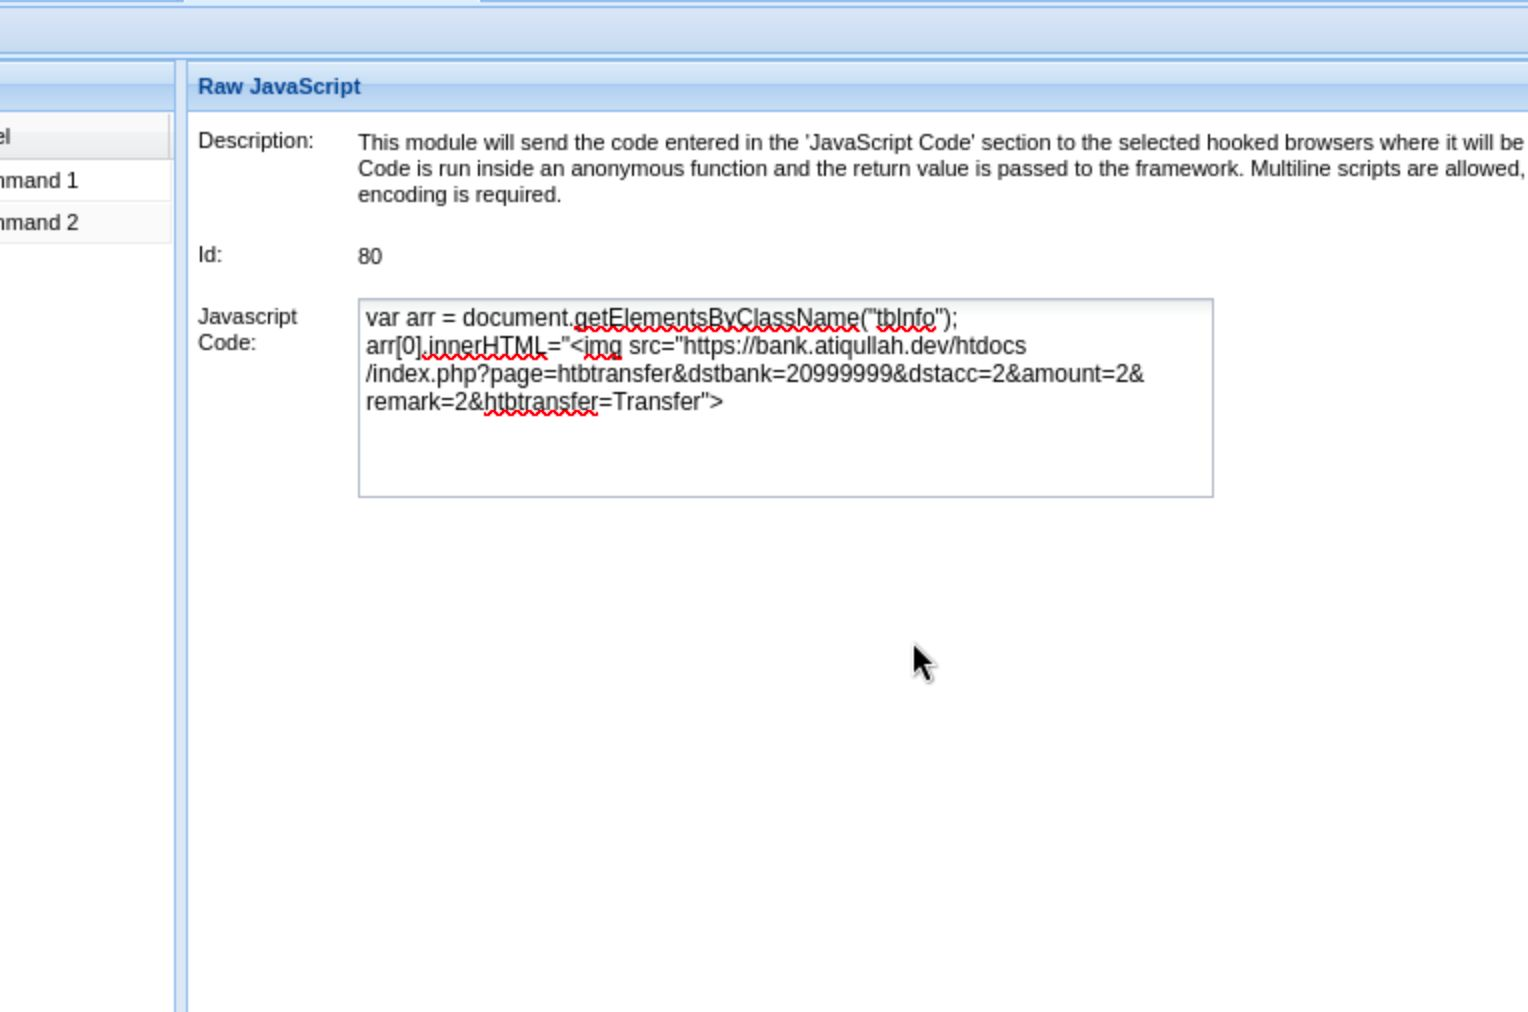
\includegraphics[width=0.7\linewidth]{alisina/beefImageTransaction.jpeg}
    \caption{Transaction through Image tag}
    \label{fig:beefImageTransaction}
\end{figure}

We forced the user with a DOM Popup to download virus.exe payload to have a backdoor attack on the user's computer. Figure \ref{fig:beefPopup} shows the attack.
\begin{figure}[H]
    \centering
    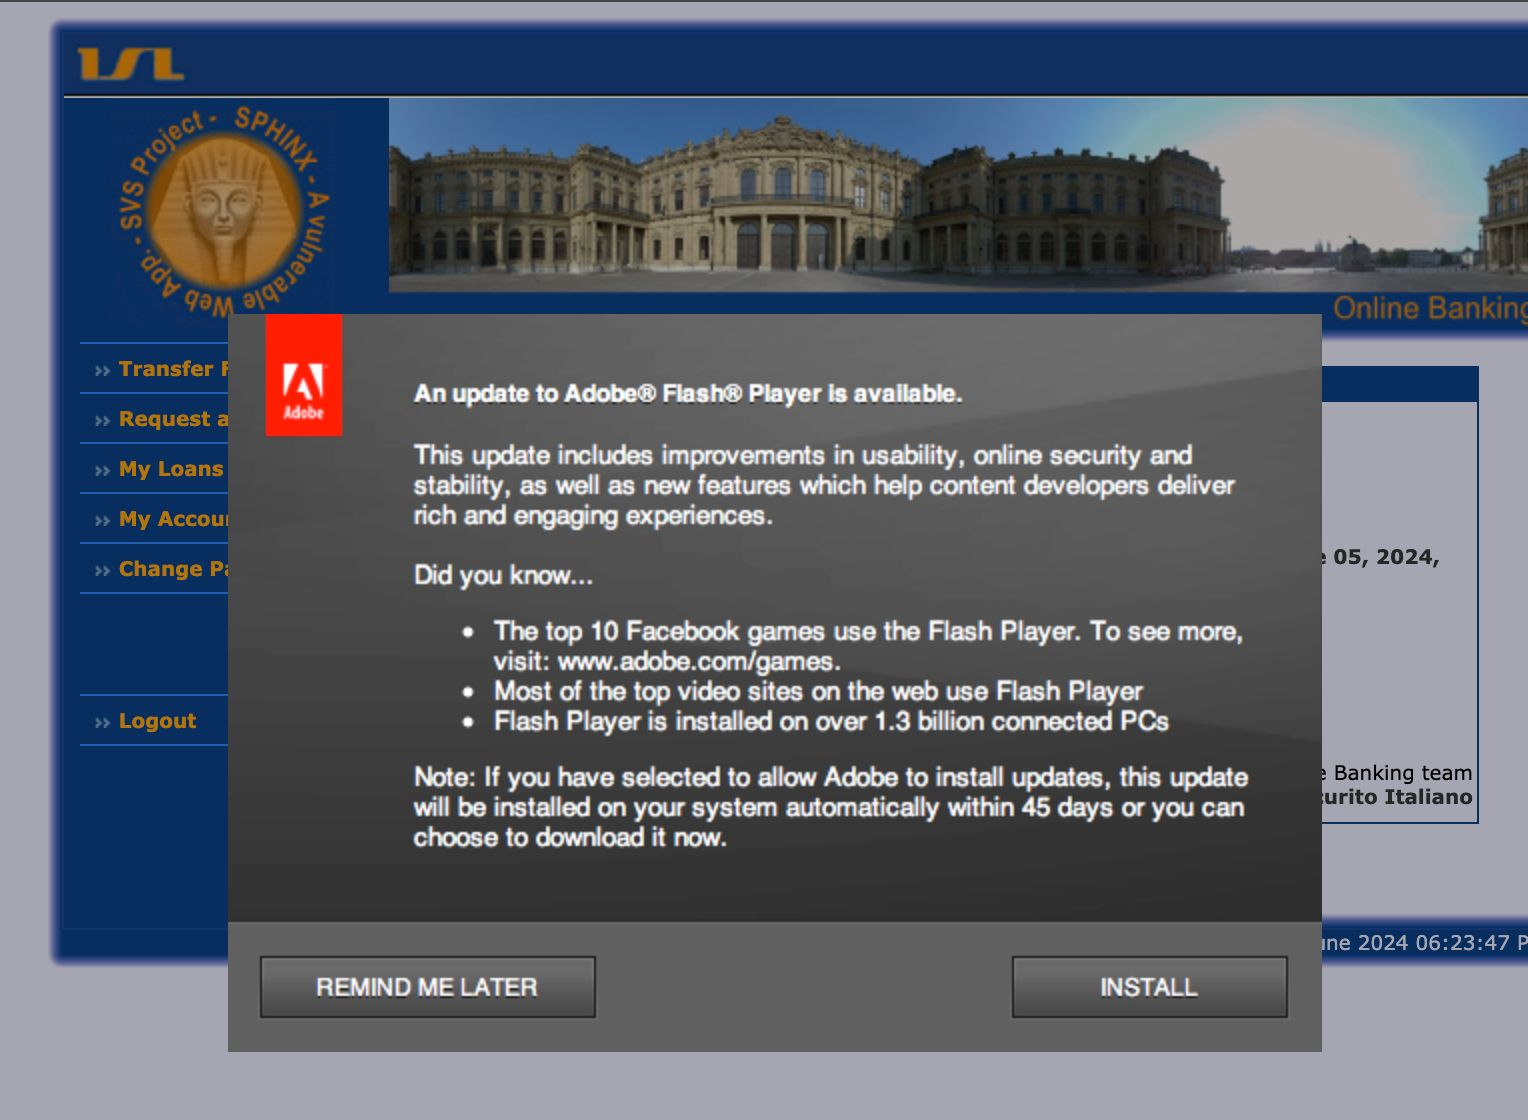
\includegraphics[width=0.7\linewidth]{alisina/beefpopup.jpeg}
    \caption{BeEF Popup example}
    \label{fig:beefPopup}
\end{figure}

In addition, we can run a DDOS attack through the victim's computer with the help of an XSS attack by running the following script.
\begin{verbatim}
 var options = {
 host: 'localhost', 
 path: '/withdraw',
 port: '1234', 
 method: 'POST',
 headers: {'Content-Type' : 'application/json'}
}; 

function readJSONResponse(response){
 var responseData = ''; 
 response.on('data', function(chunk){
 responseData += chunk;
 }); 
 response.on('end', function(){
 console.log(responseData);
 }); 
}

for( var i = 0; i < 1000; i++) {
 if(i % 2 != 0) {
 var data = {
 "amount": 0.001,
 "id": i,
 "token": dateToken
 };
 var req = http.request(options, readJSONResponse);
 req.write(JSON.stringify(data));
 req.end();
 }
}
\end{verbatim}
\nocite{sqlmap}
\nocite{zaproxy}
\nocite{burp}





